\documentclass{article}
\usepackage[a4paper,hmargin=2cm,top=2.25cm,bottom=3cm]{geometry}
\usepackage{graphicx} % Required for inserting images

\usepackage{url}
\bibliographystyle{apalike}
\usepackage{hyperref}
\usepackage[table,xcdraw]{xcolor}
\usepackage{fancyvrb}
\usepackage{minted}
\usepackage{amsmath}
\usepackage{cleveref}
\usepackage{subcaption}
\usepackage{dirtytalk}
\usepackage{parskip}
\usepackage{colortbl} 
\usepackage{multirow}
\usepackage{booktabs}
\usepackage{multicol}
\usepackage{makecell}

\usepackage{cleveref}
\usepackage{verbatim}
\usepackage{appendix}
\usepackage{listings}
\usepackage{amsfonts,amsthm}
\usepackage{tikz}
\usetikzlibrary{positioning,shapes,arrows}
\lstset{breaklines=true, basicstyle=\ttfamily}

\setlength\parskip{2ex plus 0.2ex minus 0.4ex}
\setlength\parindent{0em}

\DeclareCaptionSubType[alph]{listing}



% \title{PAR Exercise 1. Mining Robot Task.}
% \author{Andreu Garcies Ramon\\Maria Guasch Torres}
% \date{October 2025}

\title{
    \textbf{A2: Community Detection}\\
    \large Complex Networks\\
    \small Universitat Rovira i Virgili (URV)\\
    \small Master in Artificial Intelligence (MAI)
}
\author{
    Andreu Garcies Ramon\\
    \texttt{andreu.garcies@estudiantat.upc.edu}
    \and
    Maria Guasch Torres\\
    \texttt{maria.guasch.t@estudiantat.upc.edu}
}
\date{April 2026}

% \bibliographystyle{apa}

\begin{document}


\maketitle

\section{Introduction}

The aim of this report is to present the analysis of the results obtained for the second assignment of the subject. In particular, we study how community detection algorithms work in order to characterize the mesoscale of complex networks.

\section{Task 1: Characterization of the community structure of networks with block structure}\label{sec:part1}

In this first task we use community detection algorithms to analyze networks generated according to the stochastic block model (SBM). The parameters used to generate these networks are the following:

\begin{itemize}
    \item Number of nodes \texttt{N=300}.
    \item Number of different blocks of nodes \texttt{nblocks=5}.
    \item  Probability that a node, belonging to a given block, establishes a link with another node from a different block \texttt{prs=0.02}.
    \item Probability that a single node (belonging to a given block) establishes a link with another node from the same block \texttt{prr}. In this case, this indicator varies from network to network, ranging from 0 (no connections within the block) to 1 (nodes are fully connected within the block). This is what will allow us to study how these community detection algorithms work as the blocks become more and more connected within themselves.
\end{itemize}

\begin{figure}[htbp]
    \centering
    
    % Left Image: prr = 0.02
    \begin{subfigure}[b]{0.32\textwidth}
        \centering
        
\includegraphics[width=\textwidth]{assets/prr_0.02.png} % Update file name/extension
        % \caption{$p_{rr} = 0.02$}
        \label{fig:prr_002}
    \end{subfigure}
    \hfill
    % Center Image: prr = 0.16
    \begin{subfigure}[b]{0.32\textwidth}
        \centering
        
\includegraphics[width=\textwidth]{assets/prr_0.16.png} % Update file name/extension
        % \caption{$p_{rr} = 0.16$}
        \label{fig:prr_016}
    \end{subfigure}
    \hfill
    % Right Image: prr = 1.00
    \begin{subfigure}[b]{0.32\textwidth}
        \centering
        
\includegraphics[width=\textwidth]{assets/prr_1.0.png} % Update file name/extension
        % \caption{$p_{rr} = 1.00$}
        \label{fig:prr_100}
    \end{subfigure}
    
    \caption{Evolution of the network's connections as the probability of intra-block links ($p_{rr}$) increases.}
    \label{fig:network_evolution}
\end{figure}

\begin{figure}[htbp]
    \centering
    
    % Left Image: Independent Layout
    \begin{subfigure}[b]{0.48\textwidth}
        \centering
        
\includegraphics[width=\textwidth]{assets/prr_0.02_independent.png}
        \caption{Independenty applied layout algorithm}
        \label{fig:layout_independent}
    \end{subfigure}
    \hfill
    % Right Image: Anchored Layout
    \begin{subfigure}[b]{0.48\textwidth}
        \centering
        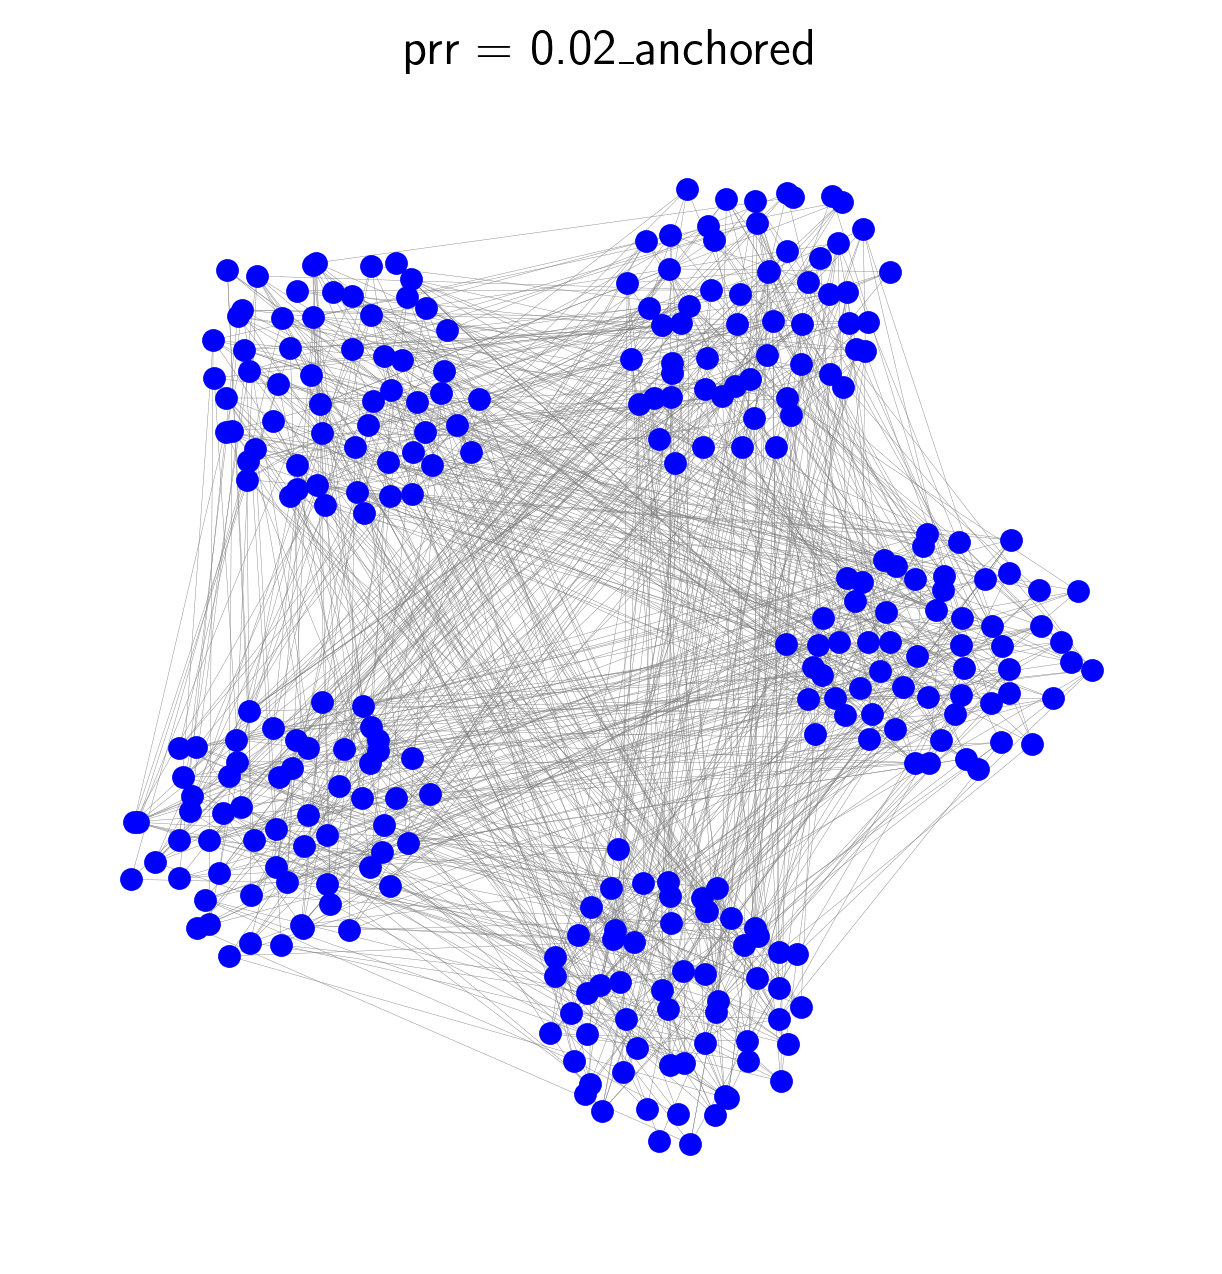
\includegraphics[width=\textwidth]{assets/prr_0.02_anchored.png}
        \caption{Anchored layout (using $p_{rr} = 1.00$)}
        \label{fig:layout_anchored}
    \end{subfigure}
    
    \caption{Comparison of visualization strategies for the sparse $p_{rr} = 0.02$ network.}
    \label{fig:layout_comparison}
\end{figure}

Figure~\ref{fig:network_evolution} shows the evolution of the connections in the network as the probability of intra-block links ($p_{rr}$) increases. At the lowest value shown in the figure ($p_{rr} = 0.02$), the actual connections within each group are very sparse. While the communities are easily distinguished in the visualization, this clustering is actually an artifact of our methodology: as requested by the project statement and to facilitate comparison between networks of different $p_{rr}$, the spatial coordinates of the nodes were anchored using a layout algorithm applied to the $p_{rr} = 1.00$ network. If we had applied it directly to the $p_{rr} = 0.02$ network, its sparse topology would make these groups nearly impossible to identify visually (as it is shown in Figure~\ref{fig:layout_comparison}). 

As the probability increases to $p_{rr} = 0.16$, the internal edges within each block become much more dense. Finally, at $p_{rr} = 1.00$, the nodes within each block form fully-connected clusters. Although we have not yet applied the community detection algorithms to the networks at this stage, this visualization clearly shows the block structure.


\subsection{Community detection algorithms}

We use three different community detection algorithms to characterize the community structure of the networks: Infomap, the Louvain method and the Agglomerative Greedy algorithm. In this section we briefly outline the theoretical foundations of each approach.

\subsubsection{Infomap}

The Infomap algorithm \cite{rosvall2009map} is an information-theoretic method for community detection. Unlike modularity maximization approaches which use the structural connection of the network, Infomap identifies communities based on network dynamics and information flow.

To model this flow, the algorithm uses a random walker navigating through the network's links. The main idea is that if a network has a well defined community structure, the random walker will spend extended periods of time trapped within certain clusters of nodes before going to other regions of the network. 

By finding the most compact way to describe the random walker's path, Infomap uses data compression to show the underlying flow of information in the network. To do so, the algorithm uses a two-level coding scheme:

\begin{enumerate}
    \item \textbf{Module Codes:} Nodes are partitioned into modules (communities). A unique index code is assigned to each module to track when the random walker transitions from one community to another.
    \item \textbf{Node Codes:} Within each module, nodes are assigned local codes. Because these local codes can be reused across different modules, the overall description of the random walker's path requires significantly less information.
\end{enumerate}

The core of the algorithm is the Map Equation, which calculates the theoretical minimum description length (in bits) required to track the path of the random walker for any given network partition. Infomap evaluates different node partitions and searches for the one that minimizes the Map Equation. The partition that gets the shortest description length represents the optimal community structure, as it best captures the regions where flow persists the longest.

For the implementation of this algorithm, we use the \href{https://mapequation.github.io/infomap/python/}{Infomap Python API}. It provides an implementation of the map equation framework.


\subsubsection{Louvain}

The Louvain method \cite{blondel2008fast} is a popular heuristic algorithm designed to extract the community structure of large networks by maximizing a metric known as Modularity ($Q$). Modularity measures the density of links inside communities compared to the expected density of links between them in a random network. A higher modularity score indicates a more defined community structure.

Unlike flow-based algorithms like Infomap, Louvain focuses entirely on the structural topology of the network. The algorithm operates in a greedy, iterative manner in two recurring phases:

\begin{enumerate}
    \item \textbf{Local optimization:} Initially, every node is assigned to its own community. The algorithm then evaluates each node and calculates the change in modularity if that node was moved into a neighboring community. The node is then placed into the community that gives the highest increase in modularity. This process is performed sequentially for all nodes, until no more node movements can improve the modularity.
    \item \textbf{Network aggregation:} Once the local optimization is done, the algorithm builds a new macroscopic network. In this new network, the communities found in the first phase become the new \say{nodes} and the links between them are formed by adding the weights of the edges between the original nodes in those respective communities.
\end{enumerate}

These two phases are repeated iteratively until the network cannot be condensed anymore and the modularity reaches its maximum value. This process makes the algorithm very computationally efficient and also provides a hierarchical community structure.

We use the \texttt{louvain\_communities} function provided by the \href{https://networkx.org/documentation/stable/reference/algorithms/generated/networkx.algorithms.community.louvain.louvain_communities.html}{NetworkX library in Python}.


\subsubsection{Agglomerative Greedy algorithm}

The Agglomerative Greedy algorithm \cite{newman2004fast, clauset2004finding} is another approach based on modularity maximization. However, unlike the Louvain method which relies on moving individual nodes to optimize modularity locally, this algorithm uses a bottom-up hierarchical clustering strategy. 

The algorithm begins with an initial state where every node in the network is assigned to its own community. From this point, it goes through an iterative agglomerative process. At each step, the algorithm evaluates all pairs of connected communities and merges the pair that results in the largest possible increase (or smallest decrease) in the overall modularity ($Q$) of the network. This merging process is repeated continuously, building larger and larger communities until all nodes in the network belong to a single community. The optimal community structure is then determined by selecting the specific partition from the merging history that corresponds to the maximum modularity value.

For the implementation of this algorithm, we use the \texttt{greedy\_modularity\_communities} function from the \href{https://networkx.org/documentation/stable/reference/algorithms/generated/networkx.algorithms.community.modularity_max.greedy_modularity_communities.html}{Python NetworkX library}.


\subsection{Analysis of the community detection results}

\begin{figure}[htbp]
    \centering
    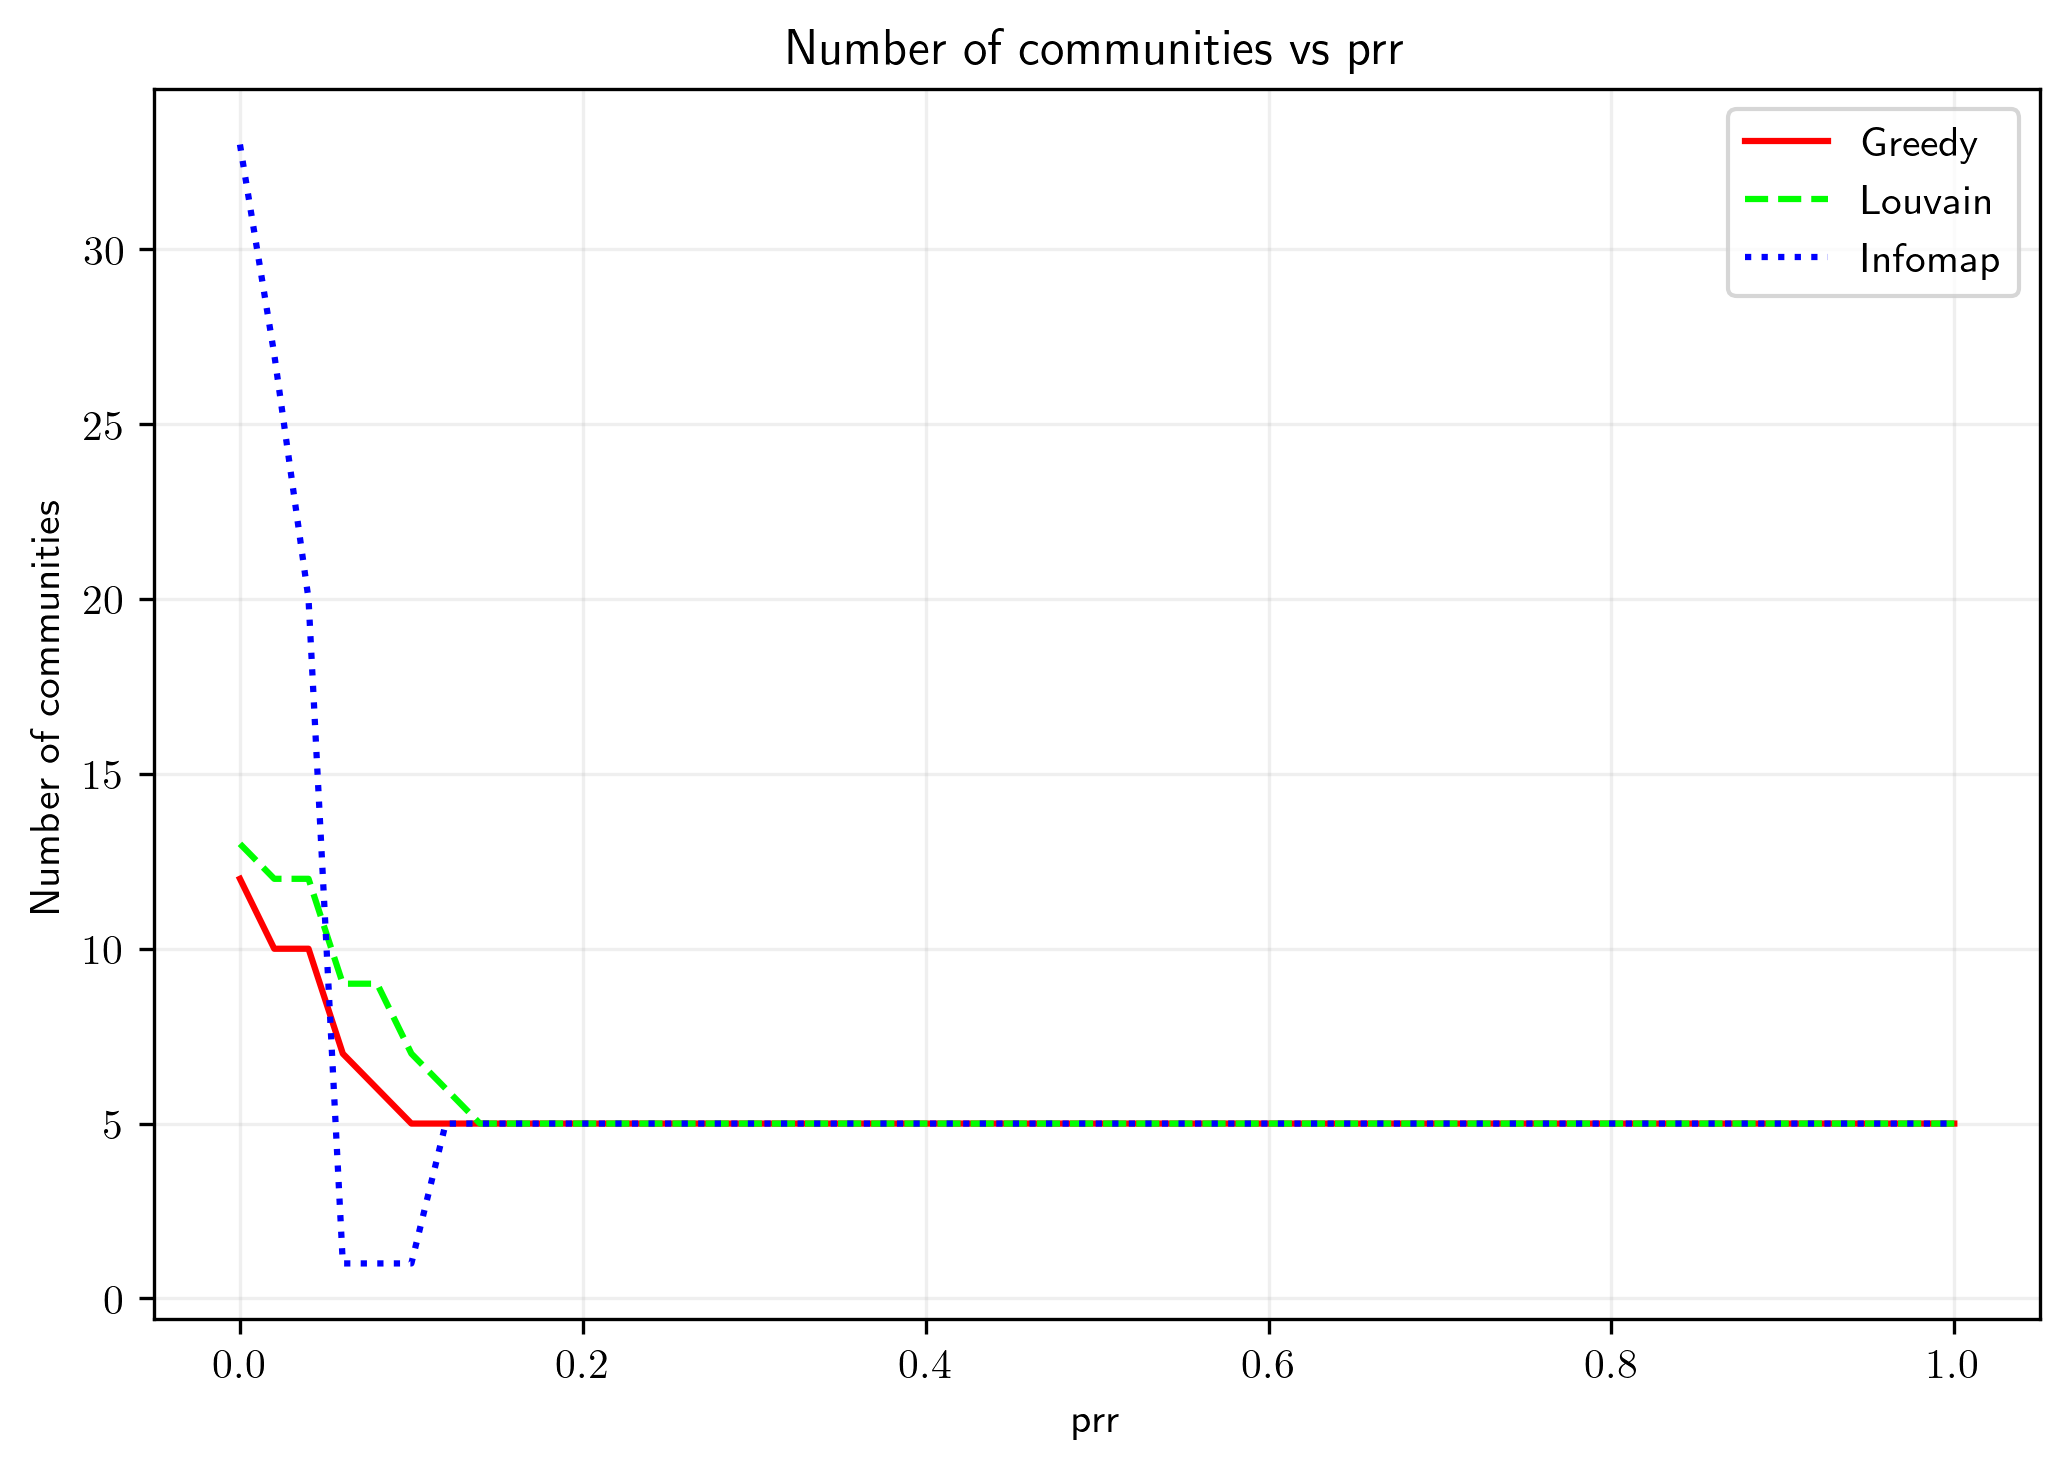
\includegraphics[width=0.6\textwidth]{assets/number_of_communities.png} 
    \caption{Evolution of number of detected communities as a function of $p_{rr}$}
    \label{fig:num_communities}
\end{figure}

\begin{figure}[htbp]
    \centering
    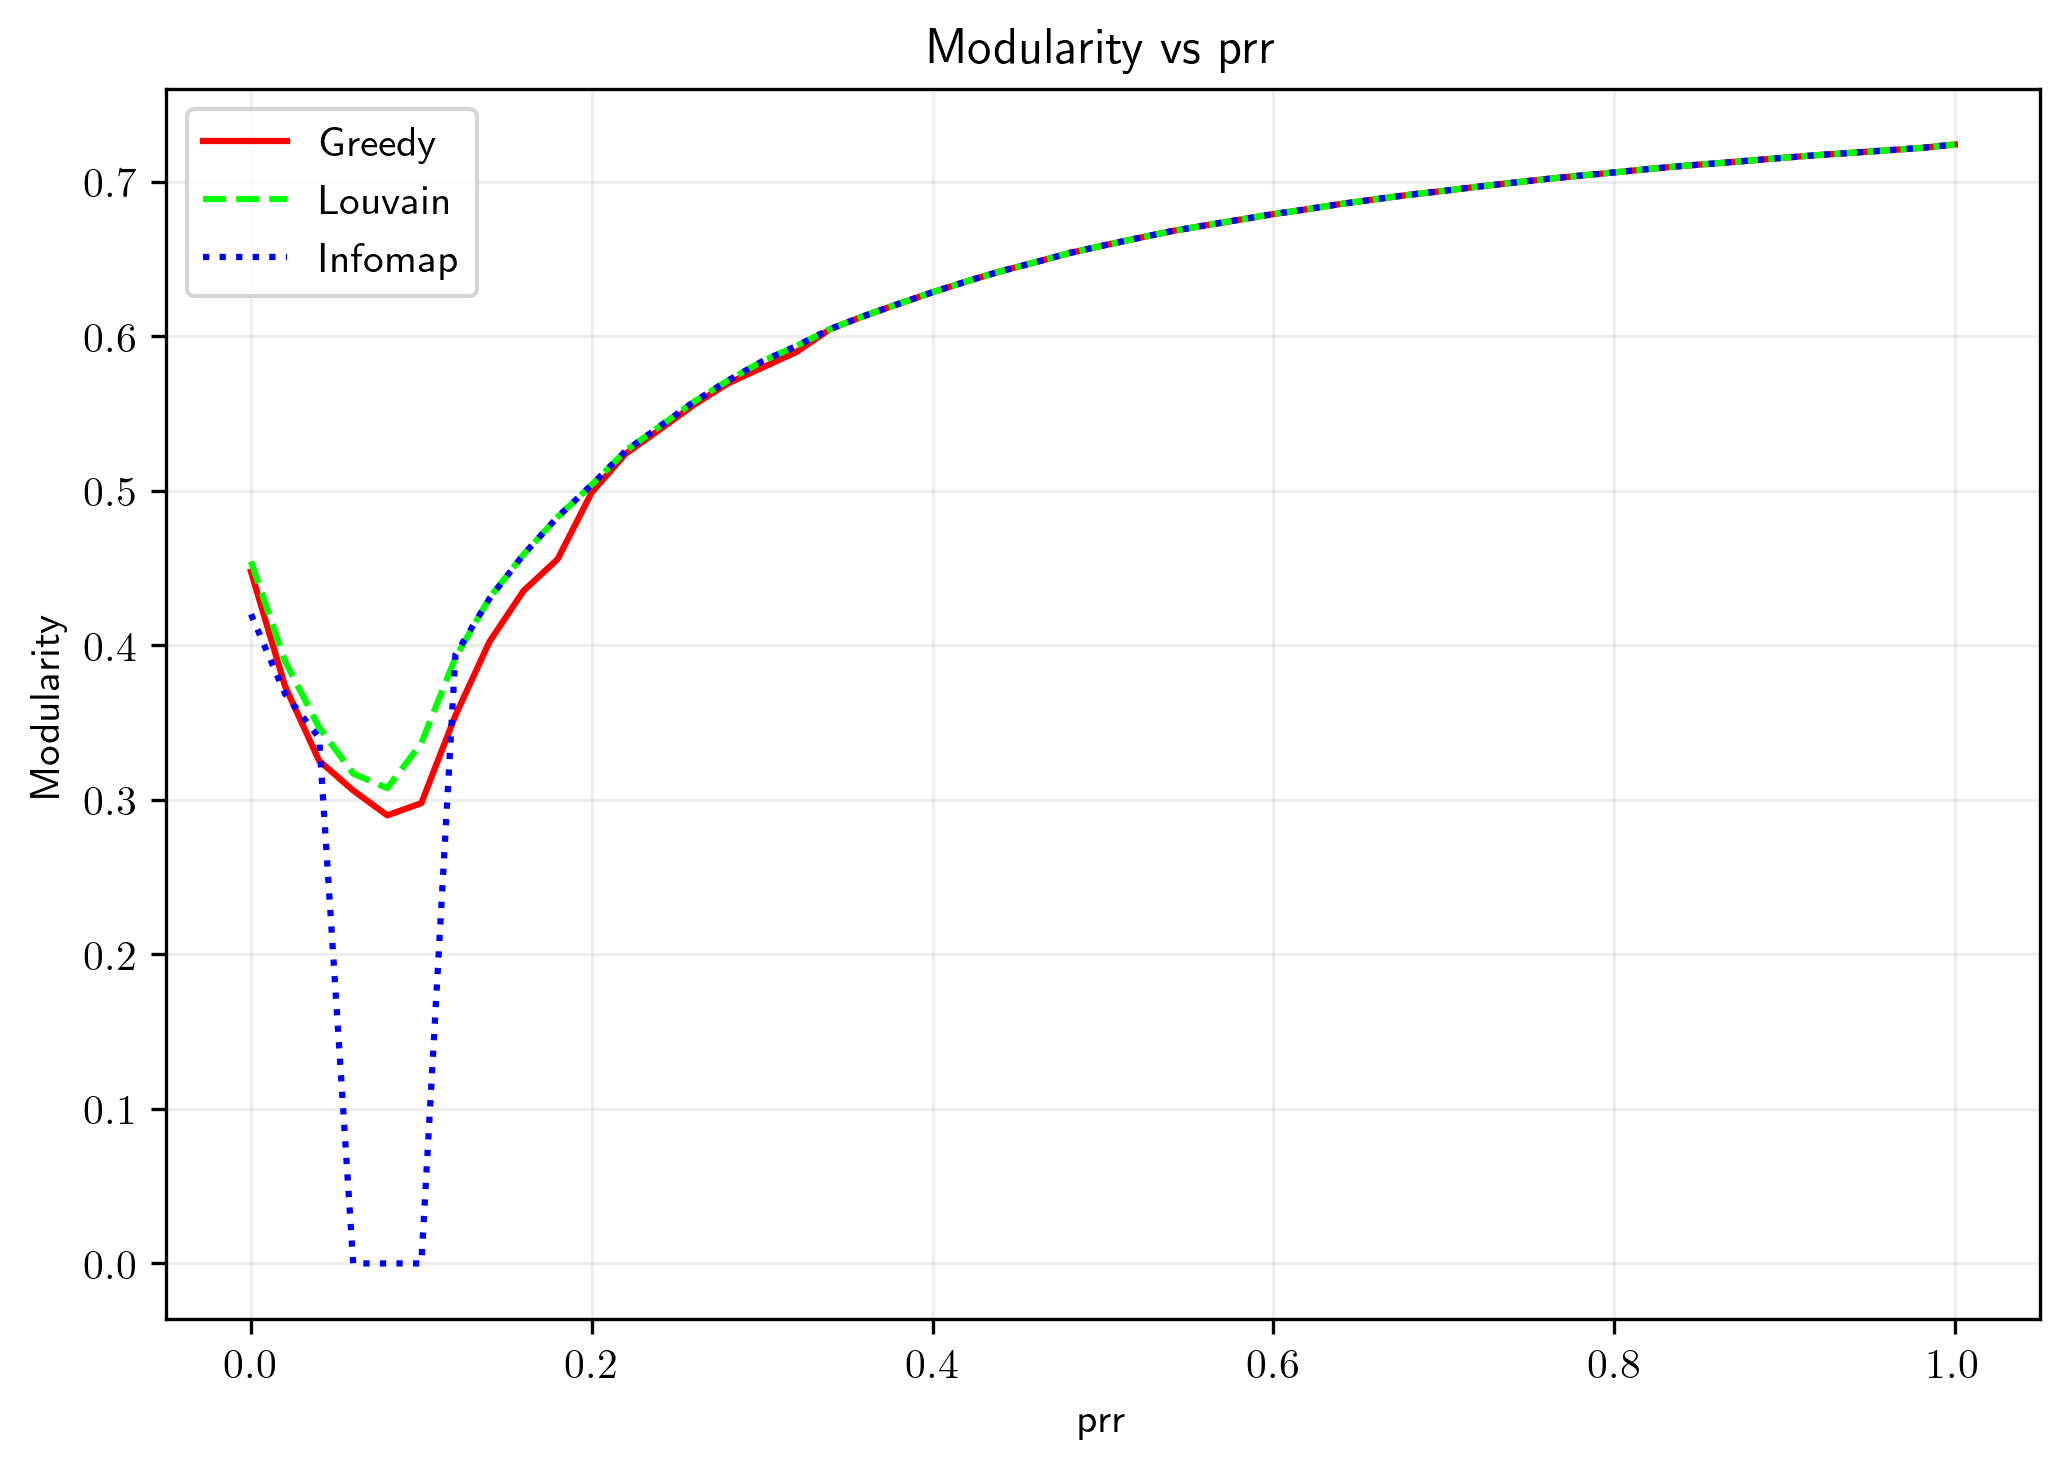
\includegraphics[width=0.6\textwidth]{assets/modularity.png} 
    \caption{Evolution of modularity as a function of $p_{rr}$}
    \label{fig:modularity}
\end{figure}

Figure~\ref{fig:modularity} shows the evolution of the modularity ($Q$) in the network as the intra-block connection probability ($p_{rr}$) increases. Both the Louvain and Agglomerative Greedy algorithms exhibit a similar plot: starting from a modularity value of around $Q = 0.45$, they then experience a slight decrease to approximately $Q = 0.3$ around $p_{rr} = 0.1$, and subsequently increasing as the network density increases as well. This alignment is expected, as both are modularity maximization algorithms and they belong to the same \say{family} of algorithms.

However, Infomap presents a slightly different evolution of modularity. Its modularity experiences a sharp drop to exactly $Q = 0.0$ between $p_{rr} = 0.05$ and $p_{rr} = 0.1$. This behavior directly correlates with the results displayed in Figure~\ref{fig:num_communities}, which show that Infomap detects exactly 1 community in this specific interval. By definition, a network partitioned into a single community that contains all nodes results in a modularity of zero.

From $p_{rr} \approx 0.15$ onwards, the three algorithms converge in both metrics. They identify the ground-truth value of 5 communities and follow an identical increasing modularity curve, reaching $Q \approx 0.7$ at $p_{rr} = 1.0$. This confirms that once the internal block structure becomes sufficiently dense, all three methods are able to correctly identify the community structure of the network.

Modularity alone is an not a reliable indicator of true community structure due to the phenomenon of \say{spurious communities}. Our results clearly demonstrate this: when $p_{rr}$ approaches 0.0, the network behaves as an Erdős-Rényi random graph with no actual communities. Yet, modularity maximization algorithms like Louvain and Greedy still report relatively high scores (approximately $Q = 0.45$). They achieve this by exploiting normal statistical fluctuations in the random distribution of edges, artificially grouping them to maximize the modularity function. Therefore, a score like $Q = 0.4$ does not guarantee a meaningful community structure—a purely random network can produce that exact same value entirely by chance.

\begin{figure}[htbp]
    \centering
    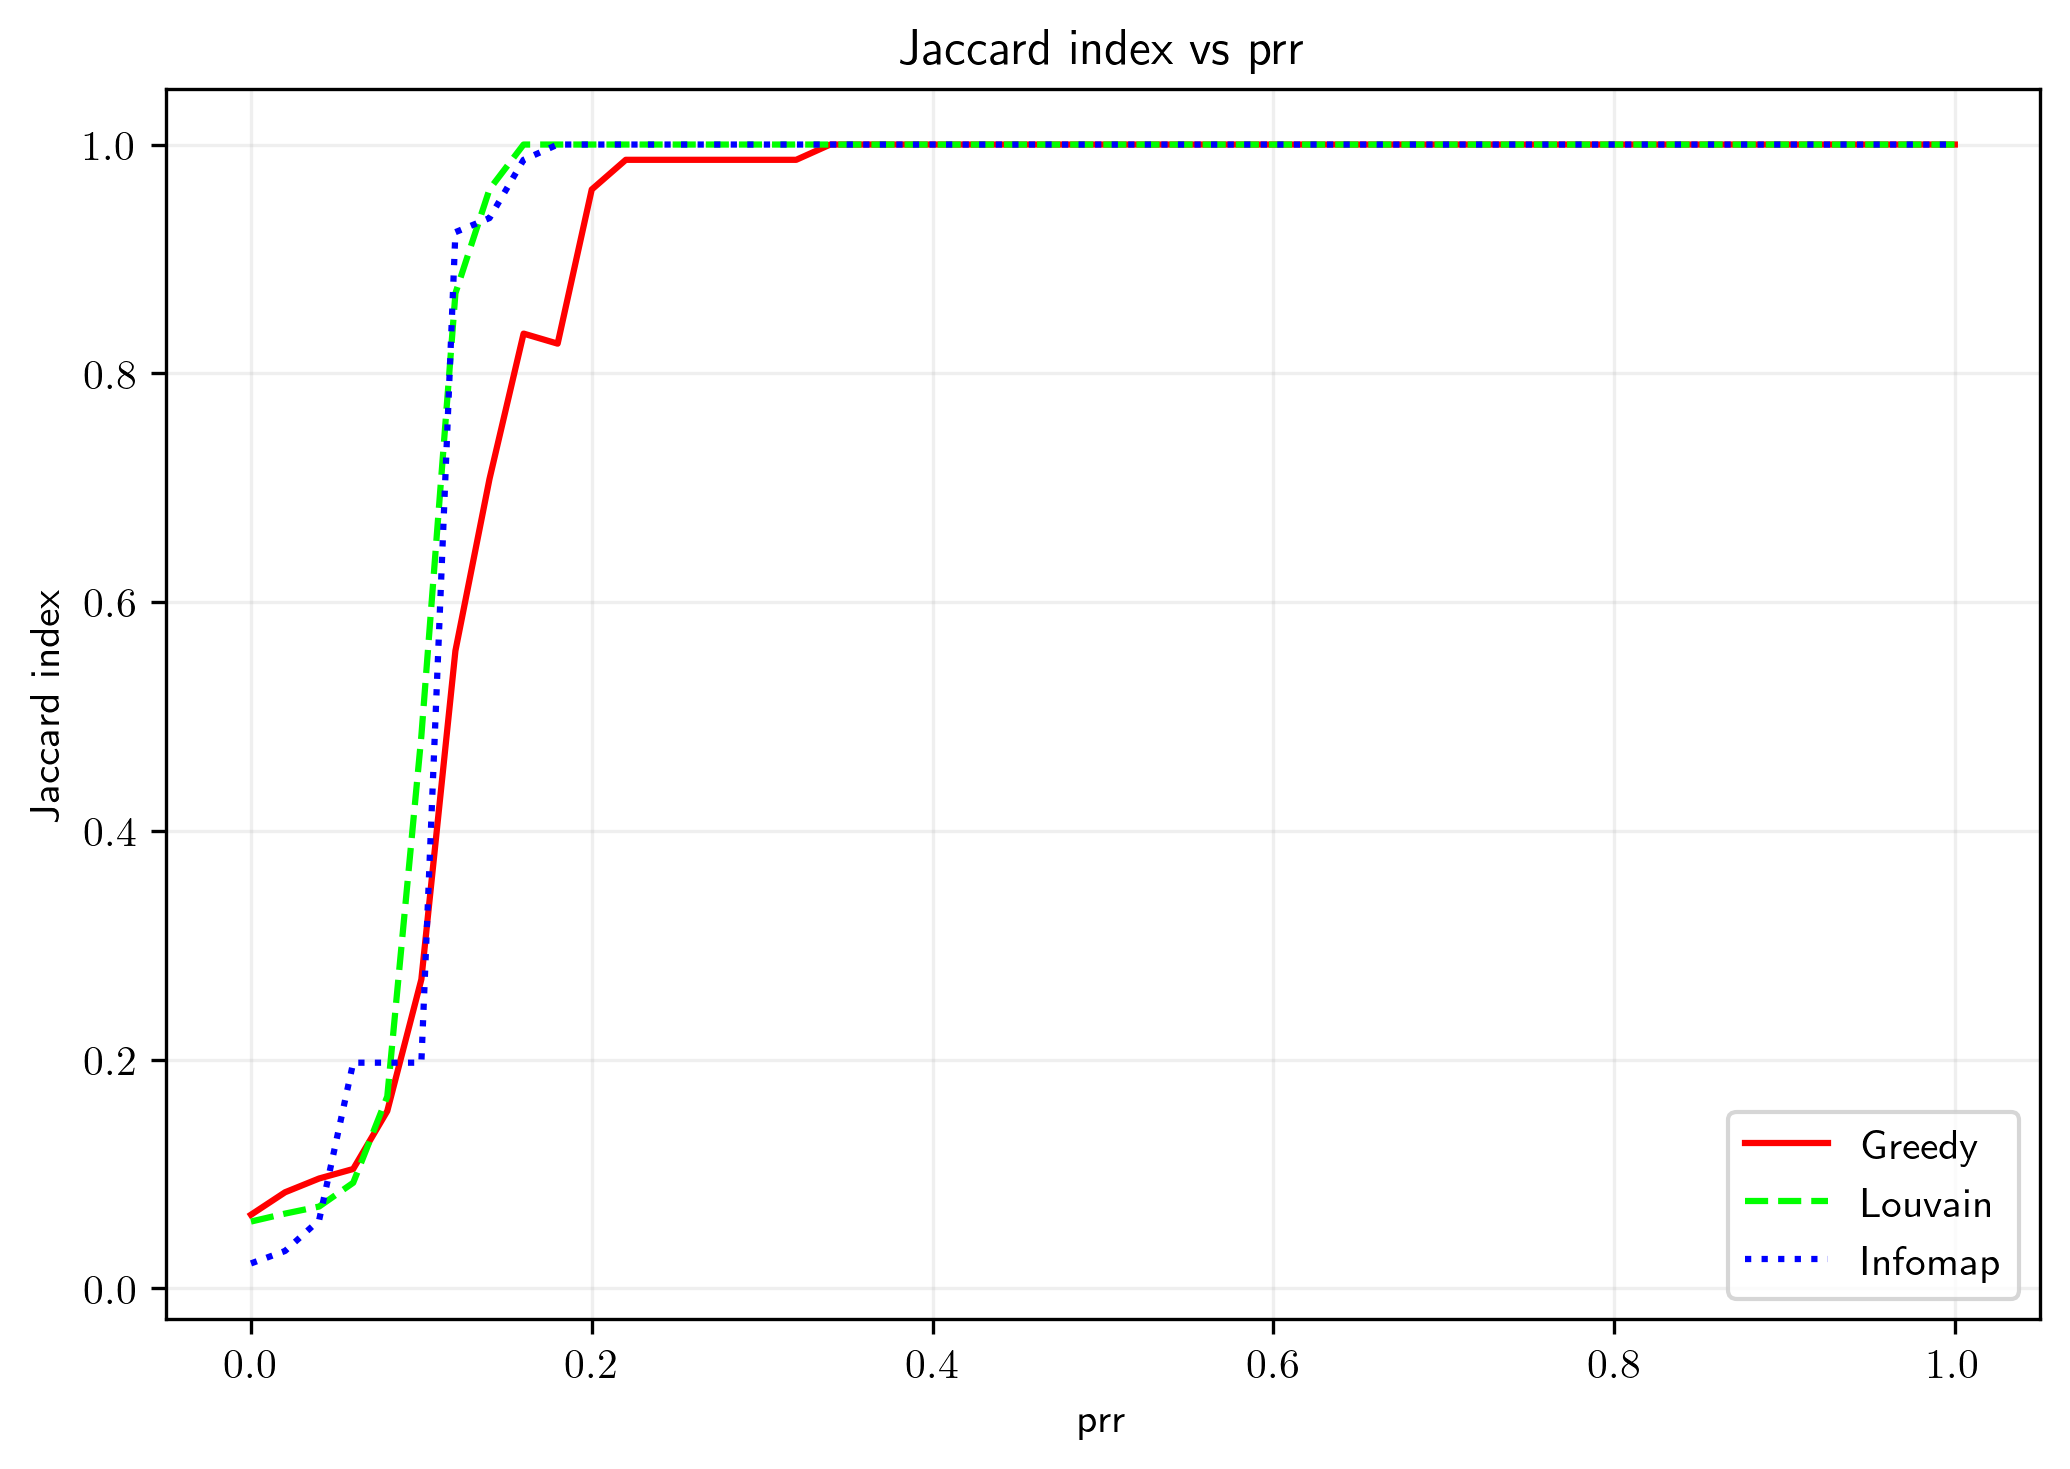
\includegraphics[width=0.6\textwidth]{assets/jaccard_index.png} 
    \caption{Jaccard index between the detected partitions and the ground truth as a function of $p_{rr}$.}
    \label{fig:jaccard}
\end{figure}

\begin{figure}[htbp]
    \centering
    
\includegraphics[width=0.6\textwidth]{assets/normalized_mutual_information.png} 
    \caption{Normalized mutual information between the detected partitions and the ground truth as a function of $p_{rr}$.}
    \label{fig:norm_mutual_info}
\end{figure}


\begin{figure}[htbp]
    \centering
    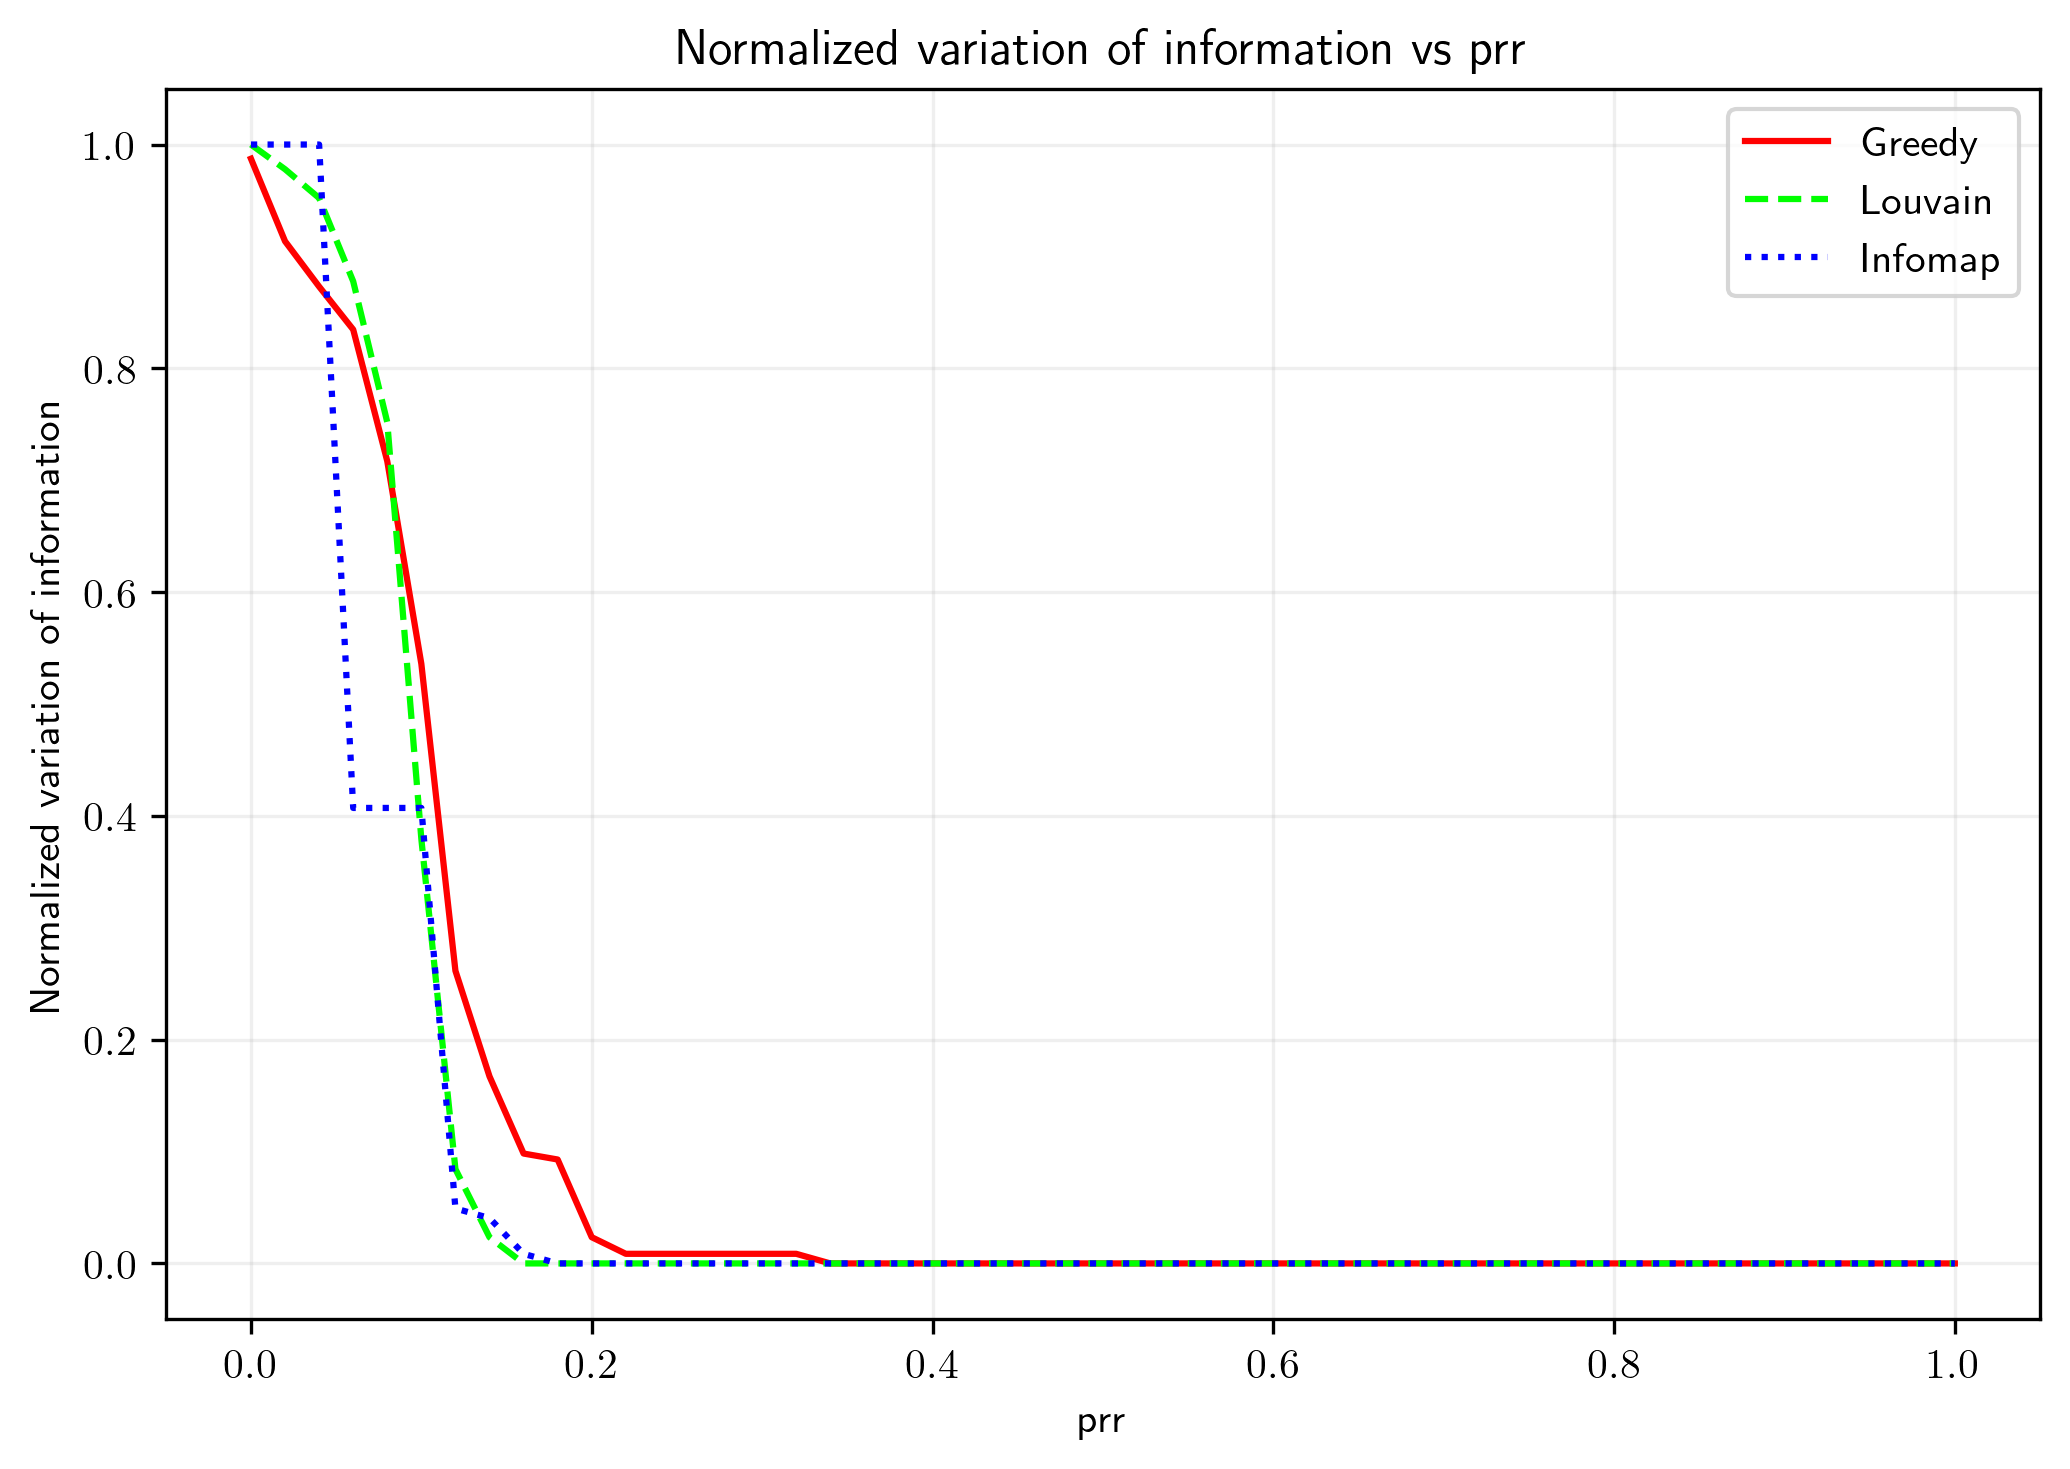
\includegraphics[width=0.6\textwidth]{assets/normalized_variation_of_information.png} 
    \caption{Normalized variation of information between the detected partitions and the ground truth as a function of $p_{rr}$.}
    \label{fig:norm_var_information}
\end{figure}

We then compare the partitions found by the algorithms against the ground-truth partition. To do so, we use three standard measures for this purpose: Jaccard Index, Normalized Mutual Information and Normalized Variation of Information.


\begin{figure}[htbp]
    \centering
    
    \begin{subfigure}[b]{0.32\textwidth}
        \centering
        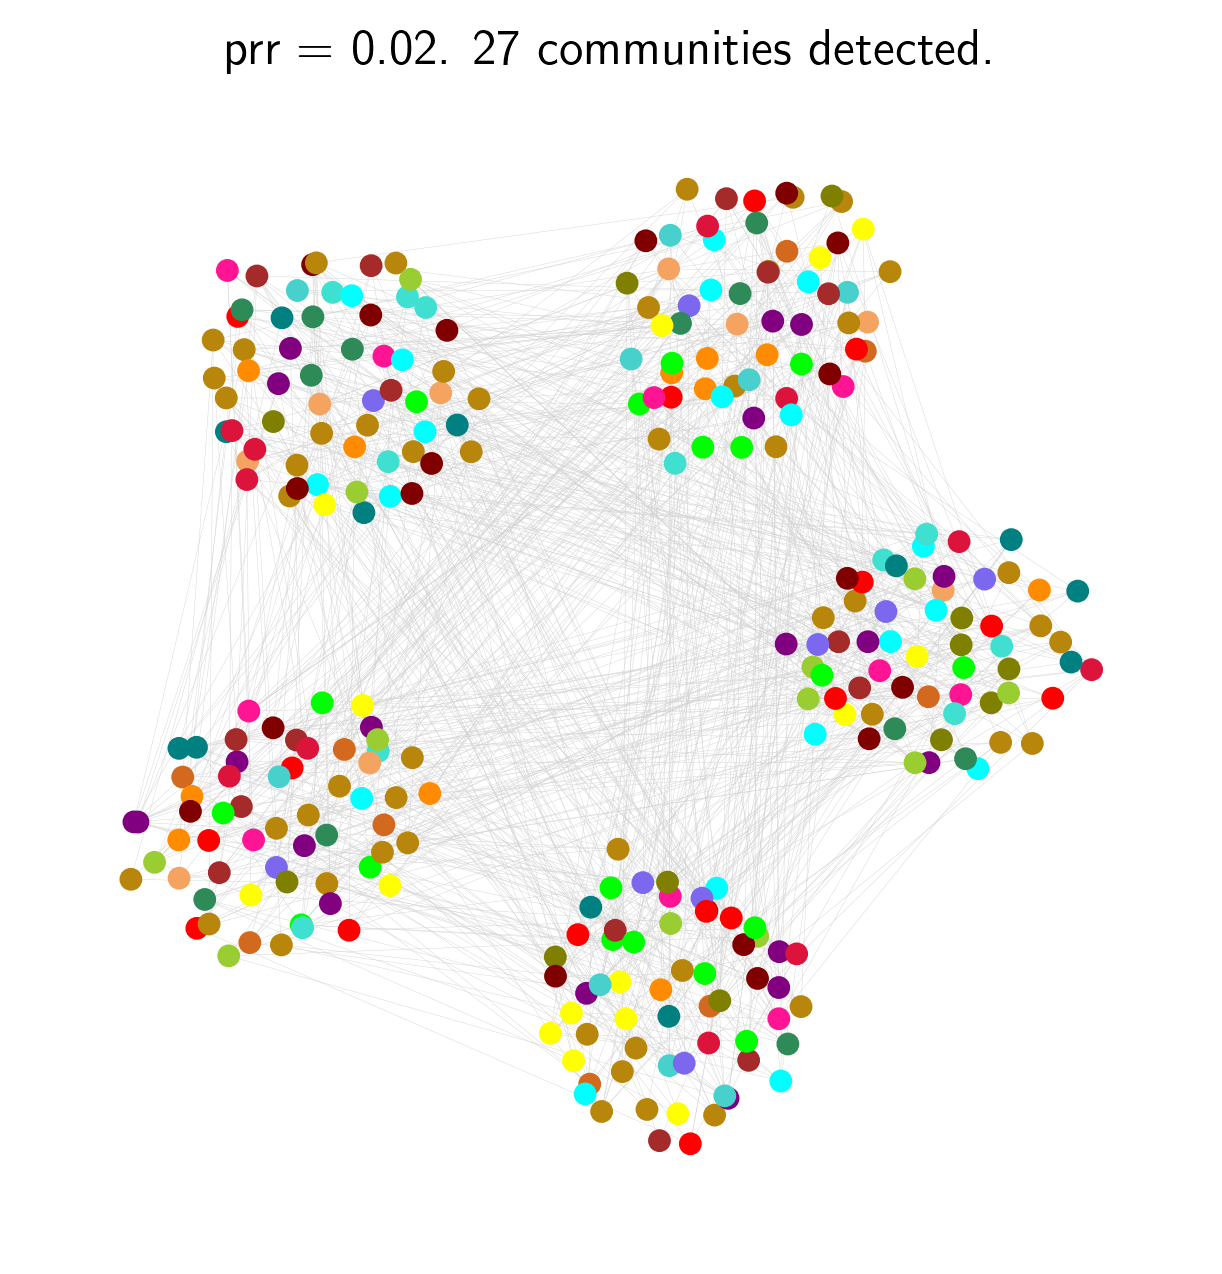
\includegraphics[width=\textwidth]{assets/prr_0.02_infomap.png} 
        % \caption{$p_{rr} = 0.02$}
        \label{fig:prr_002_infomap}
    \end{subfigure}\hfill
    \begin{subfigure}[b]{0.32\textwidth}
        \centering
        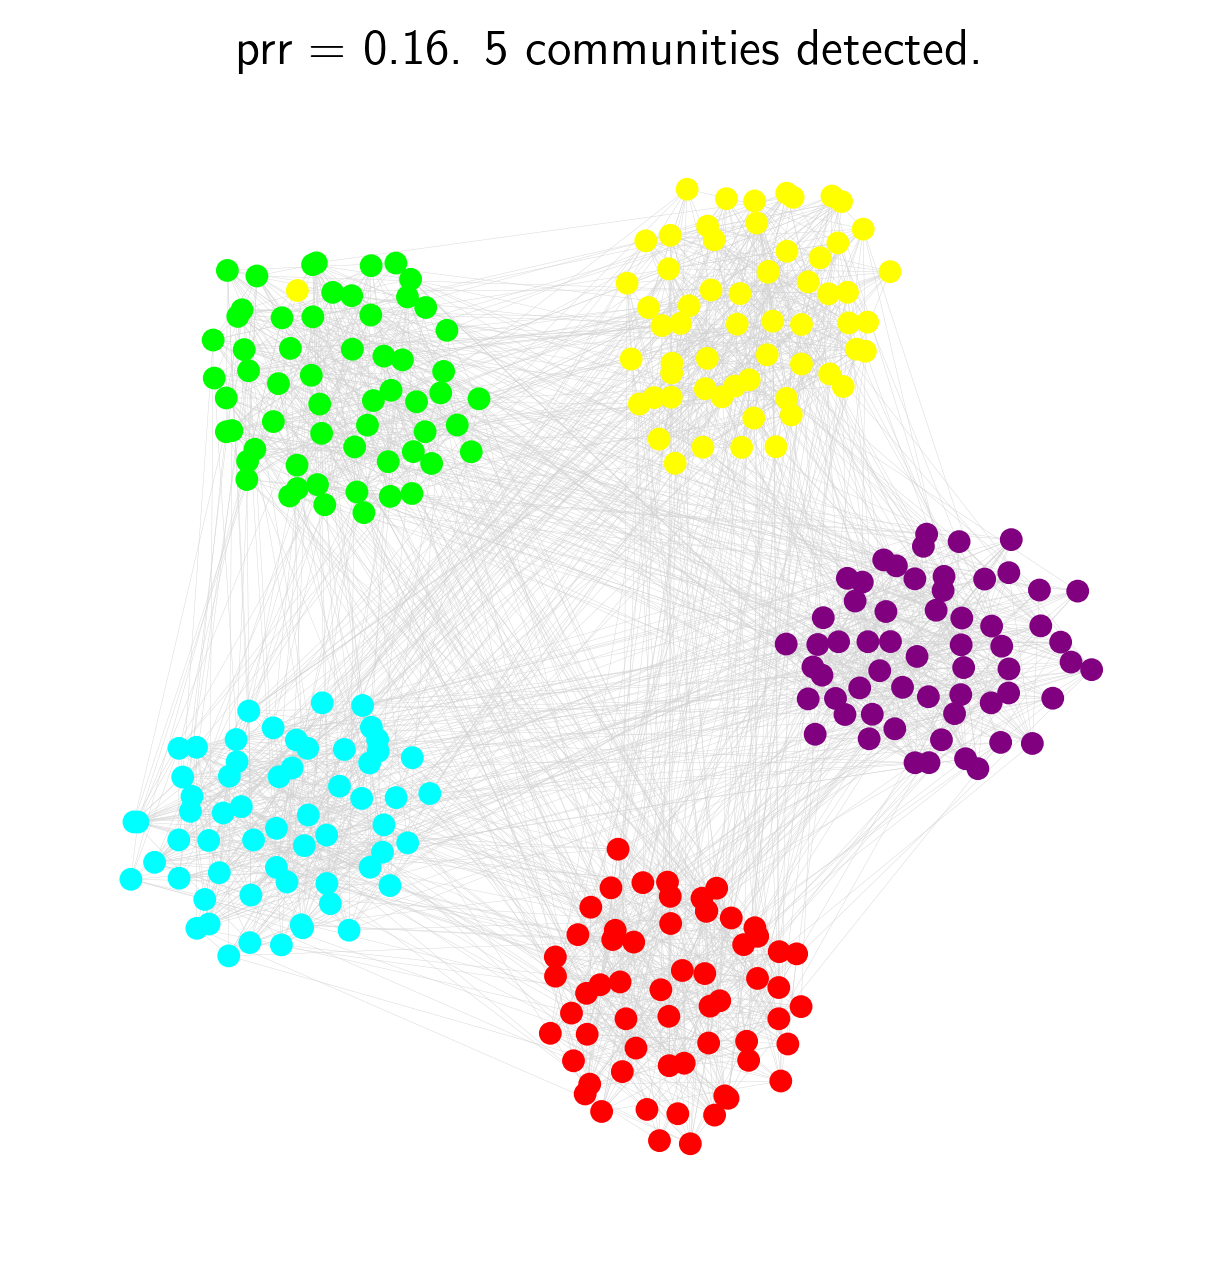
\includegraphics[width=\textwidth]{assets/prr_0.16_infomap.png}
        % \caption{$p_{rr} = 0.16$}
        \label{fig:prr_016_infomap}
    \end{subfigure}\hfill
    \begin{subfigure}[b]{0.32\textwidth}
        \centering
        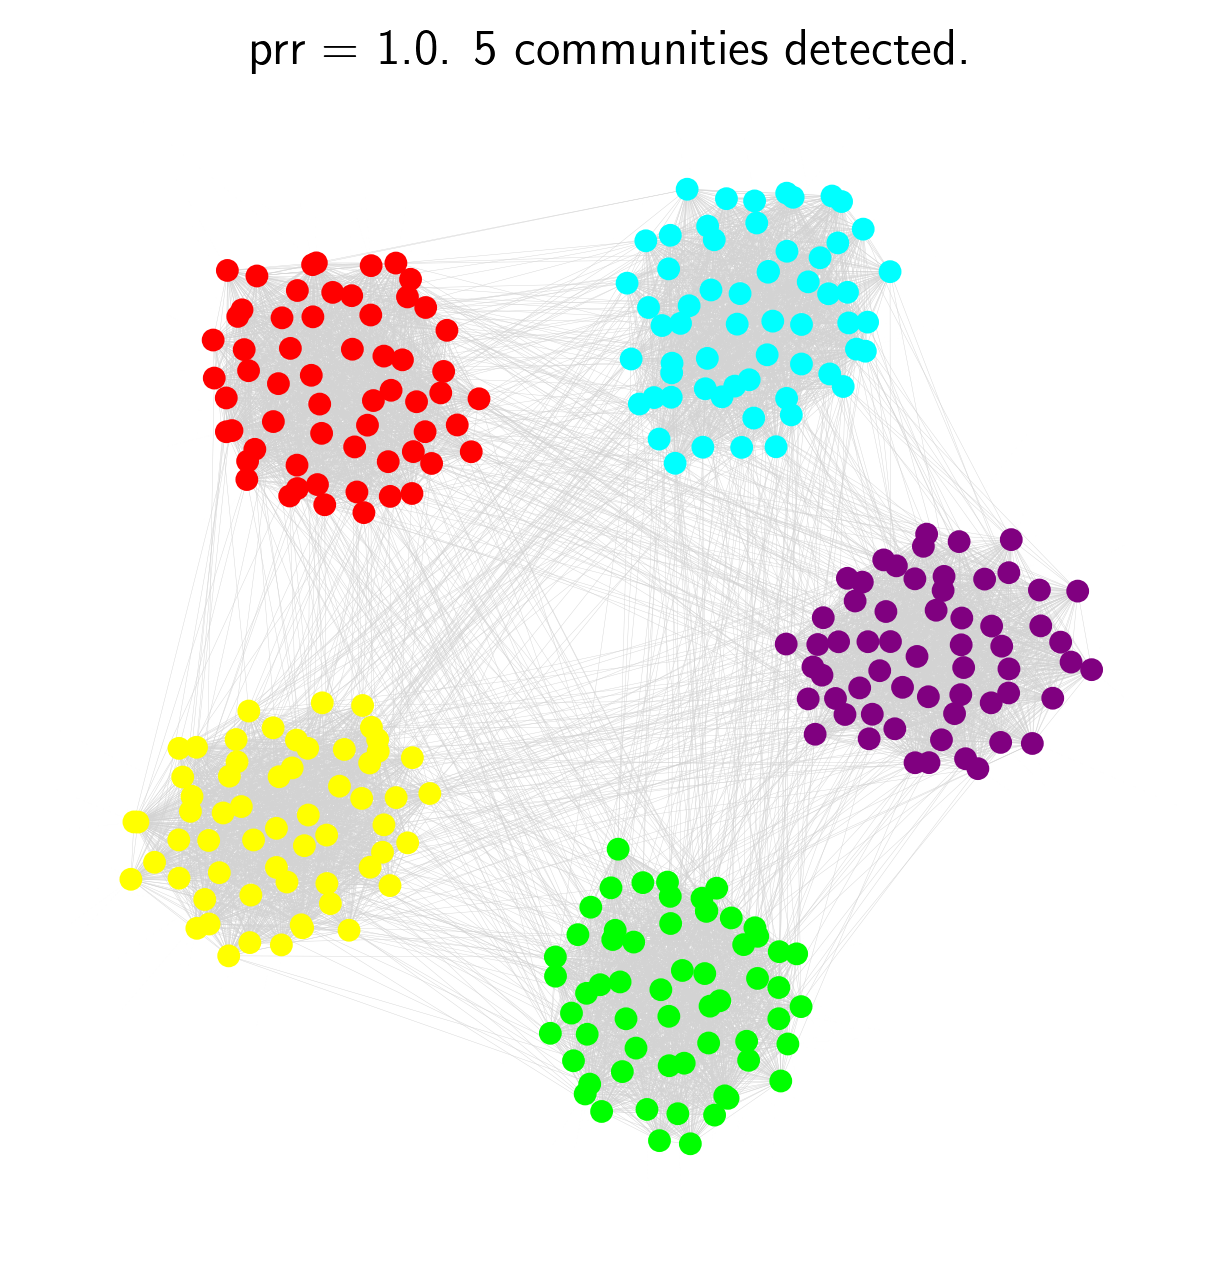
\includegraphics[width=\textwidth]{assets/prr_1.0_infomap.png}
        % \caption{$p_{rr} = 1.00$}
        \label{fig:prr_100_infomap}
    \end{subfigure}
    
    \caption{Color-coded visualization of the detected communities by the Infomap algorithm}
    \label{fig:community_detection_infomap}
\end{figure}


\begin{figure}[htbp]
    \centering
    
    \begin{subfigure}[b]{0.32\textwidth}
        \centering
        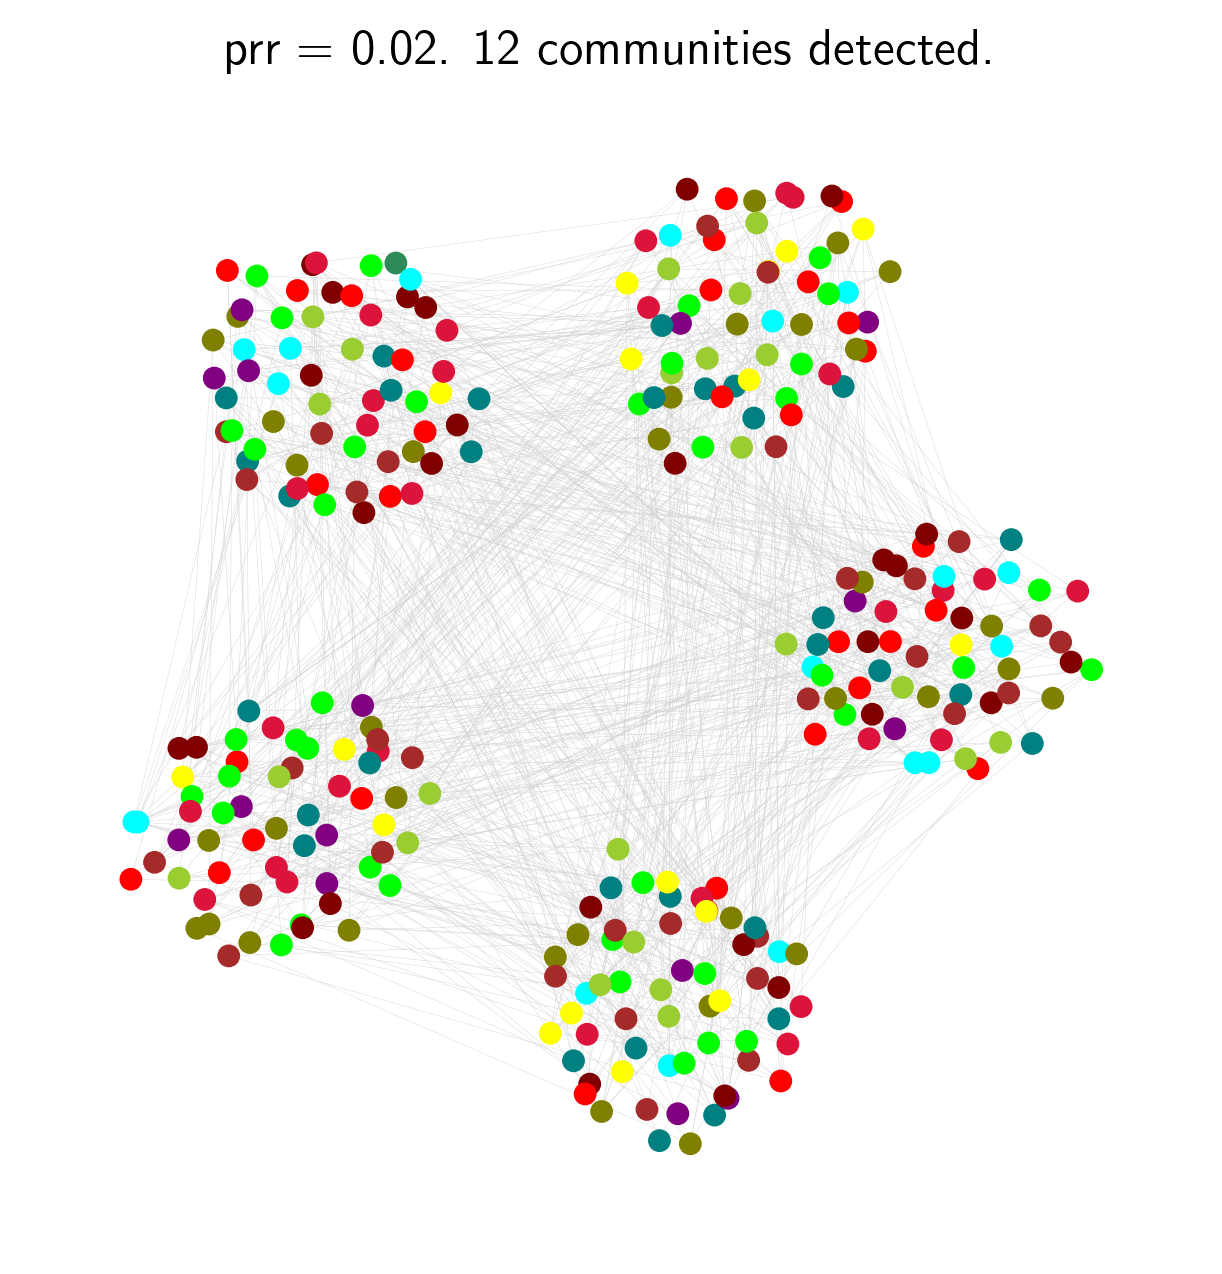
\includegraphics[width=\textwidth]{assets/prr_0.02_louvain.png} 
        % \caption{$p_{rr} = 0.02$}
        \label{fig:prr_002_louvain}
    \end{subfigure}\hfill
    \begin{subfigure}[b]{0.32\textwidth}
        \centering
        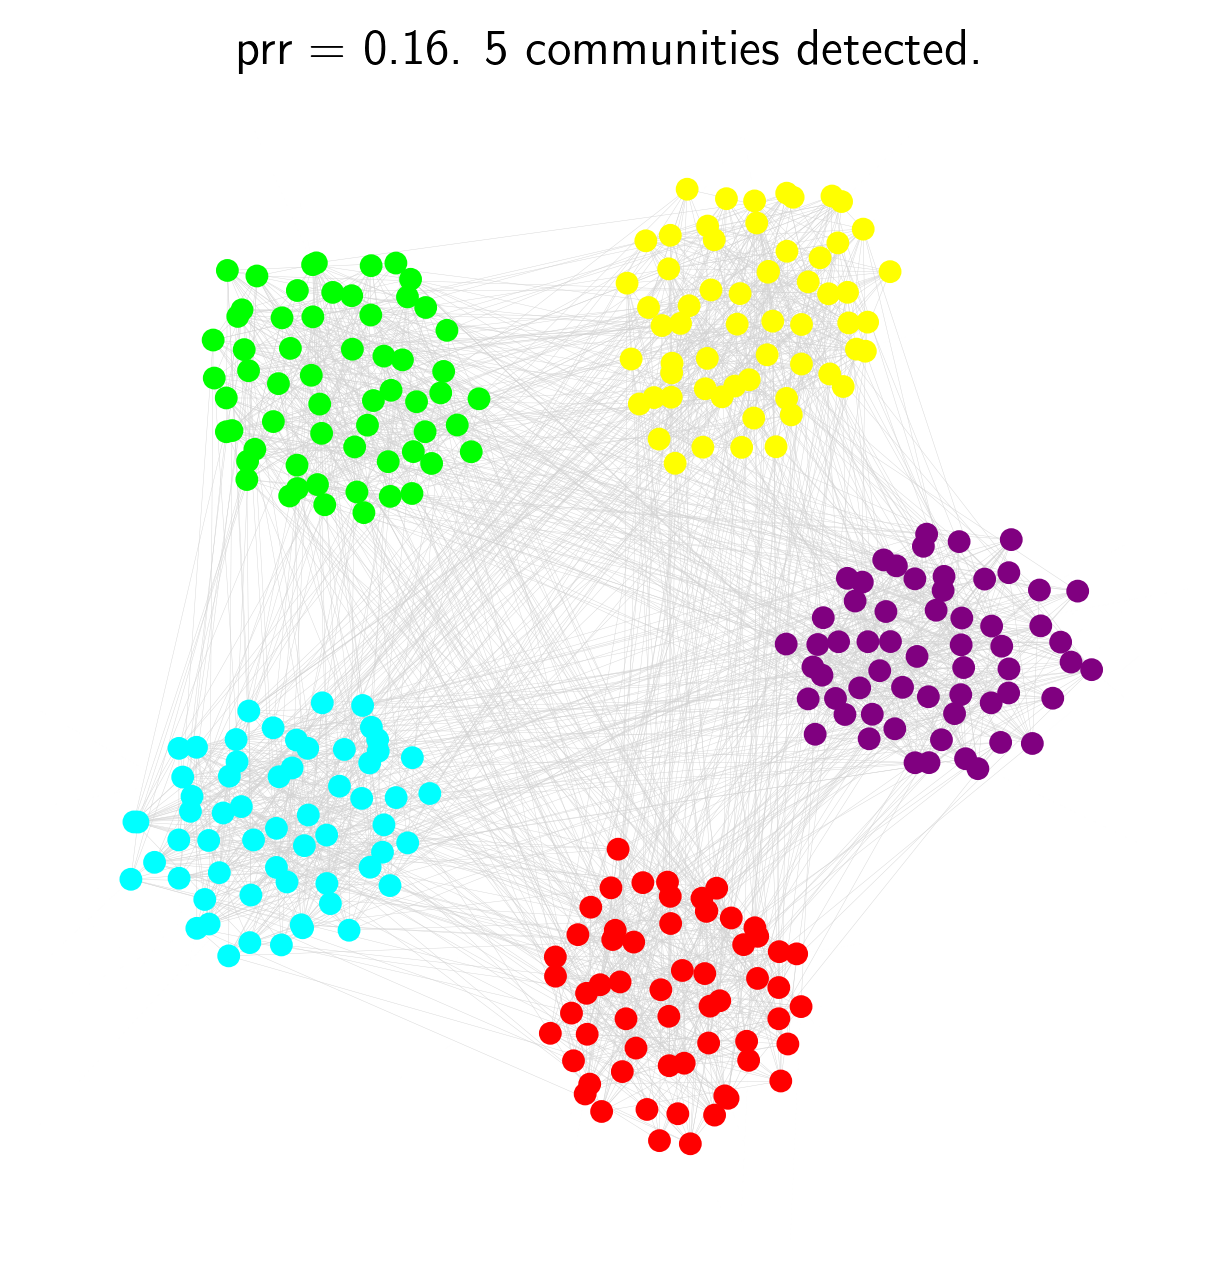
\includegraphics[width=\textwidth]{assets/prr_0.16_louvain.png}
        % \caption{$p_{rr} = 0.16$}
        \label{fig:prr_016_louvain}
    \end{subfigure}\hfill
    \begin{subfigure}[b]{0.32\textwidth}
        \centering
        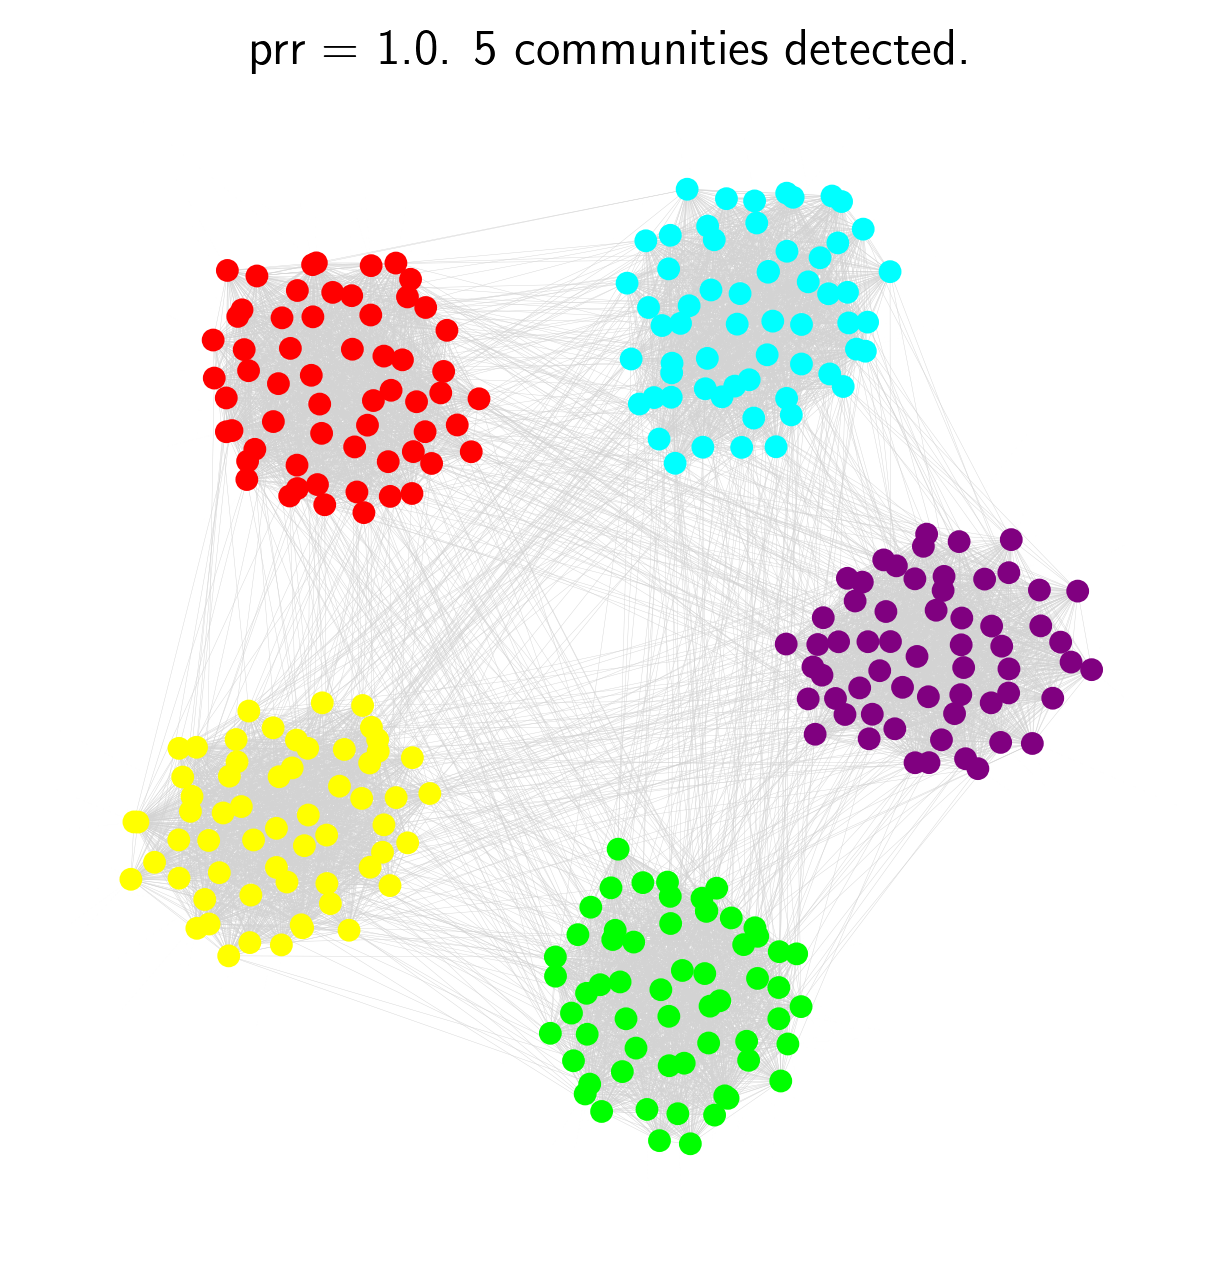
\includegraphics[width=\textwidth]{assets/prr_1.0_louvain.png}
        % \caption{$p_{rr} = 1.00$}
        \label{fig:prr_100_louvain}
    \end{subfigure}
    
    \caption{Color-coded visualization of the detected communities by the Louvain algorithm}
    \label{fig:community_detection_louvain}
\end{figure}


\begin{figure}[htbp]
    \centering
    
    \begin{subfigure}[b]{0.32\textwidth}
        \centering
        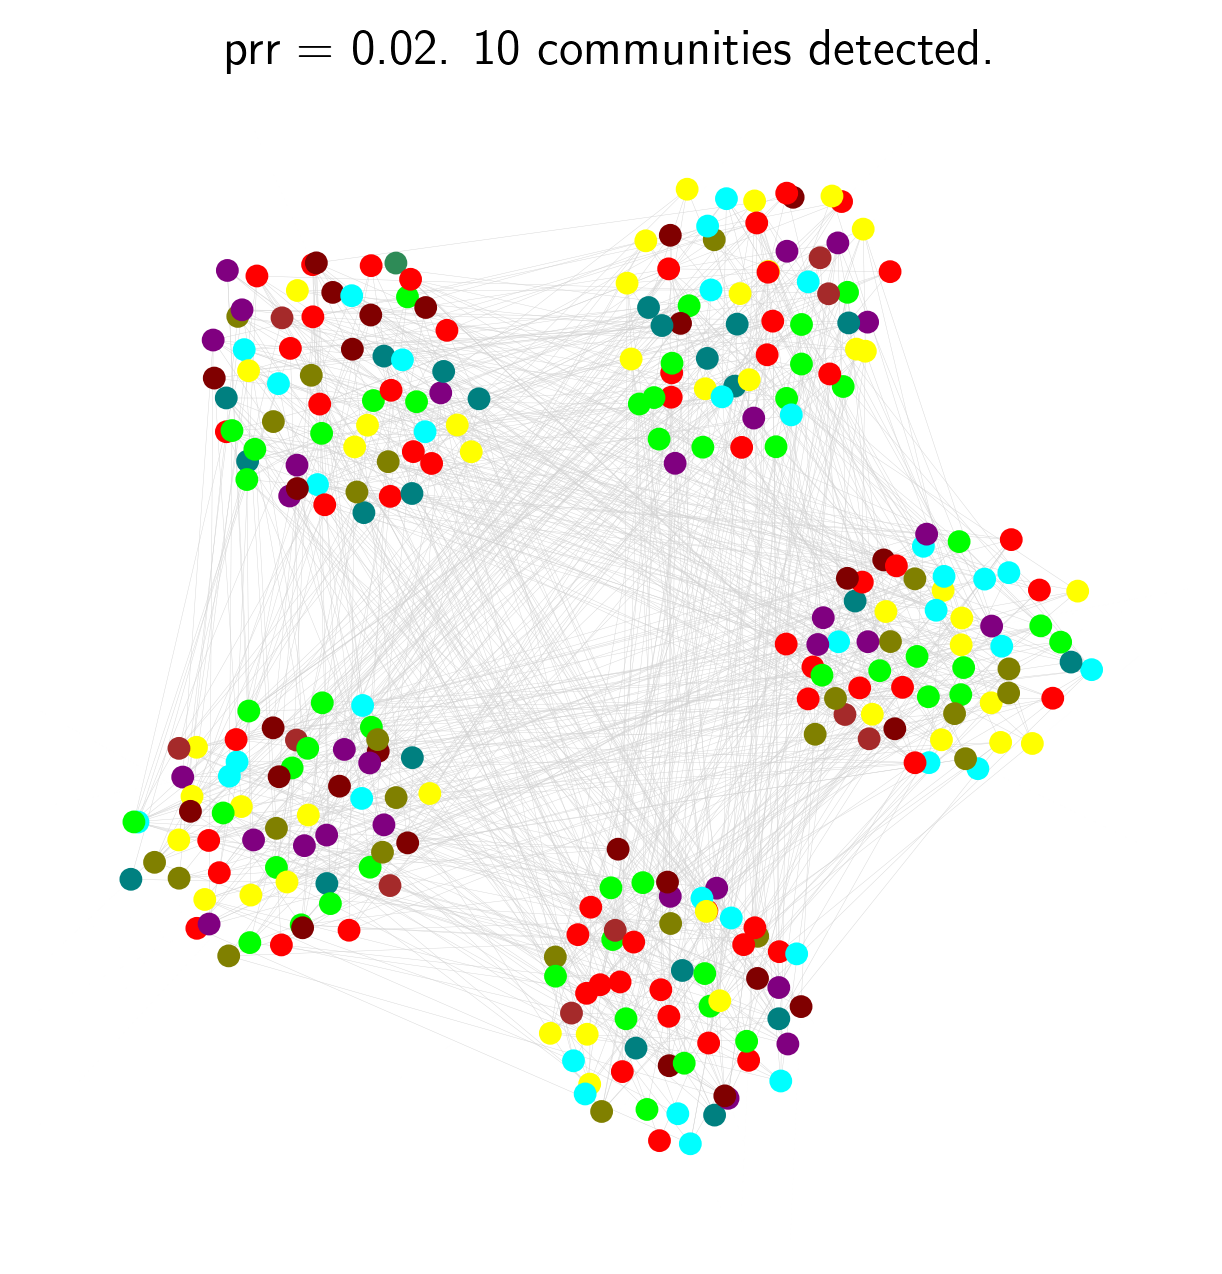
\includegraphics[width=\textwidth]{assets/prr_0.02_greedy.png} 
        % \caption{$p_{rr} = 0.02$}
        \label{fig:prr_002_greedy}
    \end{subfigure}\hfill
    \begin{subfigure}[b]{0.32\textwidth}
        \centering
        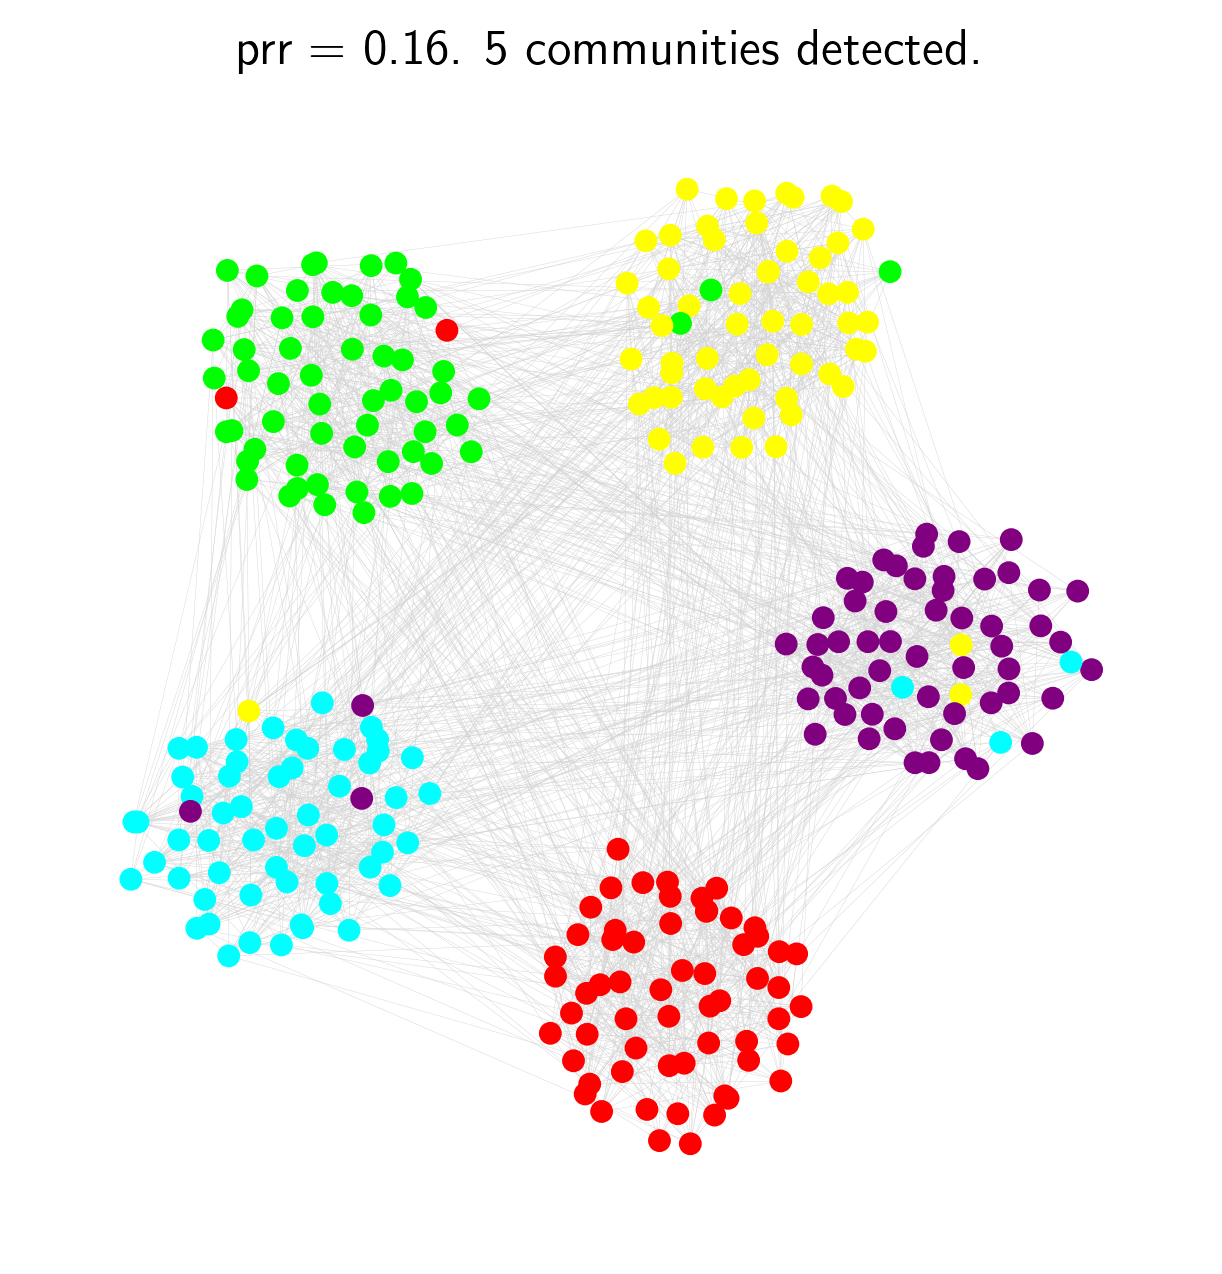
\includegraphics[width=\textwidth]{assets/prr_0.16_greedy.png}
        % \caption{$p_{rr} = 0.16$}
        \label{fig:prr_016_greedy}
    \end{subfigure}\hfill
    \begin{subfigure}[b]{0.32\textwidth}
        \centering
        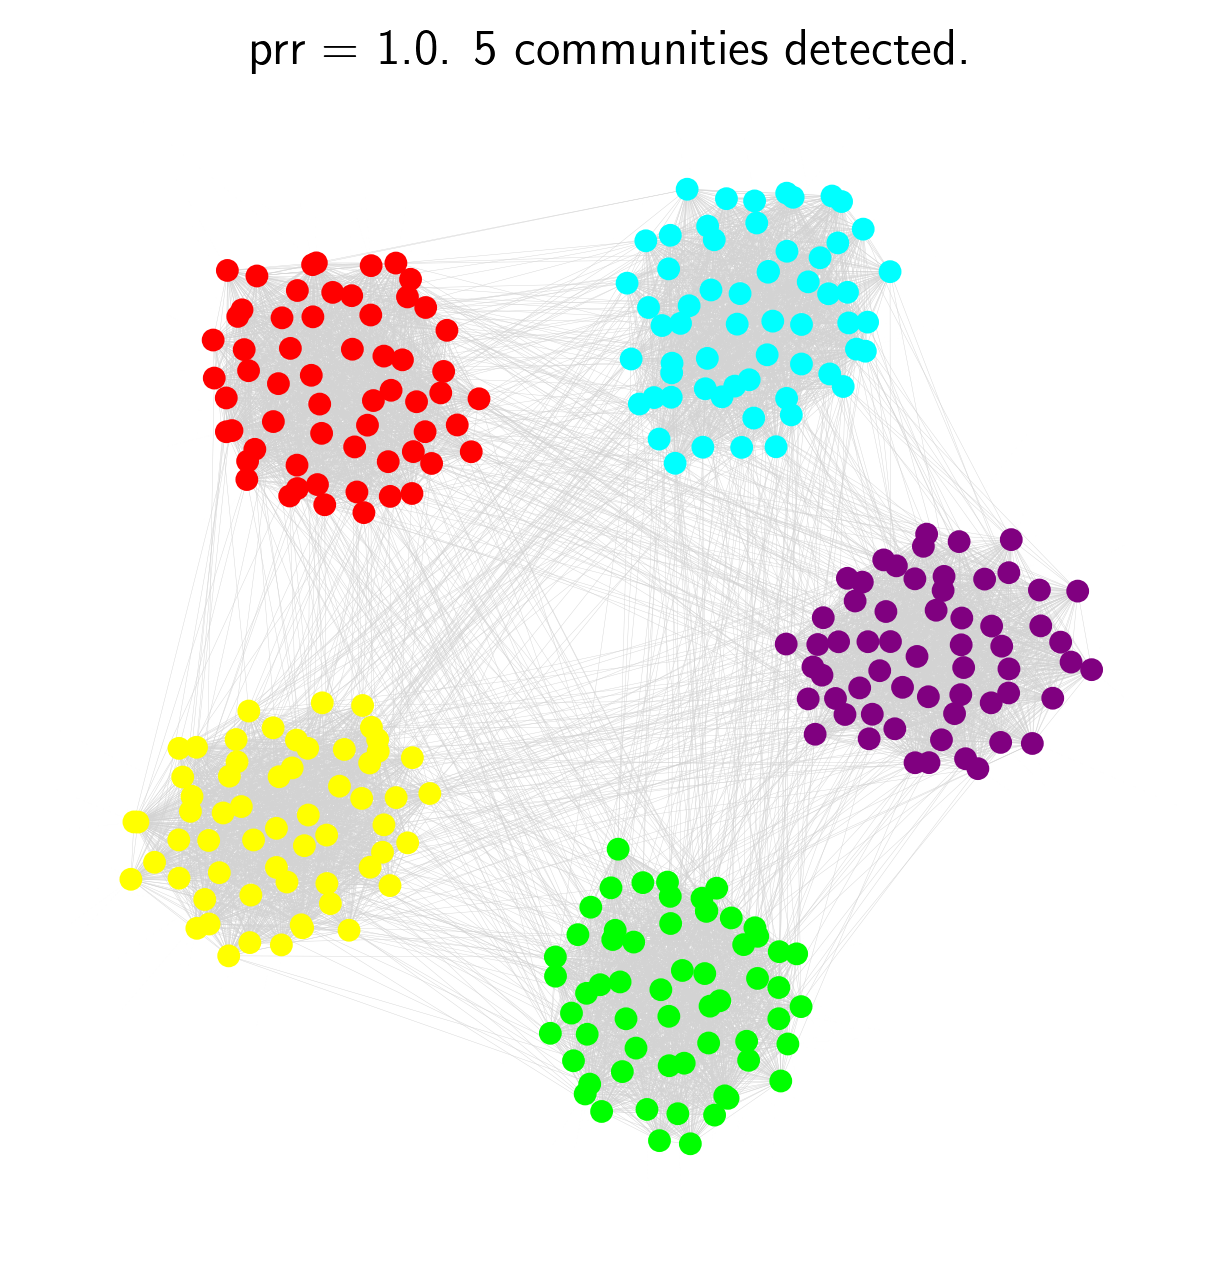
\includegraphics[width=\textwidth]{assets/prr_1.0_greedy.png}
        % \caption{$p_{rr} = 1.00$}
        \label{fig:prr_100_greedy}
    \end{subfigure}
    
    \caption{Color-coded visualization of the detected communities by the Agglomerative Greedy algorithm}
    \label{fig:community_detection_greedy}
\end{figure}


\section{Task 2: Characterization of the community structure of real networks}



\section{Conclusions}

In this report, we have shown how the structural descriptors provide powerful tools for understanding the organization of complex networks. By combining macroscopic and microscopic analyses, we have been able to distinguish between homogeneous and heterogeneous topologies, identify the presence of hubs, and evaluate the small-world properties. We have associated each network with its corresponding generative model, and the simulations generated suggest that these models have been correctly matched to their respective networks.

For the fifth network, a different approach has been followed, leading to the exploration of a model not covered in the theoretical lectures. In particular, a spatial model based on node positions has been proposed as a possible mechanism to generate the network.

\newpage
\bibliography{references}

\clearpage

% \appendix

% \section{Rule definition prompt}\label{sec:prompt}
% This section includes the prompt used to generate the initial set of rules for our fuzzy expert system using DeepSeek.
% \lstinputlisting{prompt.txt}

\end{document}
